\subsection{MIMO радиолокация}\label{sect:mimo-theory}

Рассмотрим структуру классической антенной решётки, показанную на Рисунке~\ref{fig:antenna-array-interference}. 

Сигнал образованный в каждом направлении пространства (либо полученный с него) является суммой 
излучений/принятых сигналов с каждого антенного элемента.

\begin{equation*}
    E=\sum_{1}^{N} E_n
\end{equation*}

\noindent где $E_n$ находится по уравнению~(\ref{eqn:antenna-array-element-value}).

Диаграммообразование в классических антенных решёток выполняется за счёт синфазного сложения сигналов с разных каналов. 
Установка соответствующего комплексного коэффициента передачи для каждого канала формирует соответствующий волновой фронт 
(угол наклона относительно плоскости антенной решетки) в дальней зоне излучения антенны (либо, соответственно, принимает его). 

Говоря о радиолокации, можно утверждать, что приёмник (как цифровой так и аналоговый), получают информацию о цели из 
фаз сигнала, наведённого на приёмные антенны. Аналогично передающая решётка формирует наибольшее усиление в 
определённом направлении за счёт установки соответствующих фаз в каналах. 

Таким образом, приёмная решётка изменяет коэффициенты в каналах так, чтобы сигнал от цели, который приходит на элементы 
с разной фазой, стал синфазным, а передающая - таким образом, чтобы сигналы от разных каналов 
были приняты на цели с одинаковой фазой. 

Если же передающая решётка будет излучать синфазный сигнал со всех каналов, то у цели они будут приняты, 
и отражены с разной фазой. Если каким-то образом отметить и разделить сигналы от разных каналов передающей решётки, 
то на приёмной можно будет установить направление на цель относительно передающей решётки. 

Общая идея MIMO радиолокаторов заключается в том, что как передающая, так и приёмная решётка являются цифровыми.
Таким образом MIMO радиолокатор представлен множеством антенн, 
которые передают и принимают сигнал независимо друг от друга. 
Затем принятые сигналы проходят совместную обработку для построения множества диаграмм направленности.

\begin{figure}[H]
    \centering
    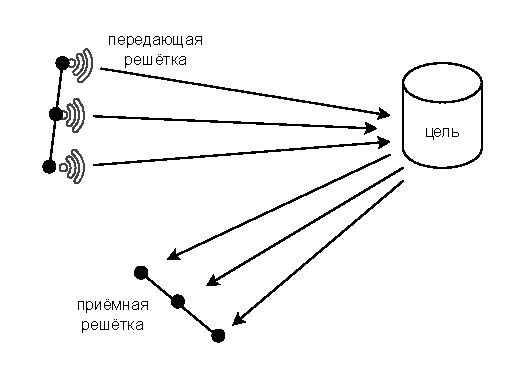
\includegraphics[width=0.8\textwidth,height=0.35\textheight,keepaspectratio]{MIMO-Demo}
    \caption{Иллюстрация MIMO радиолокатора. Положения как приёмных и передающих каналов известны в общем центре обработки данных}%
    \label{fig:mimo-demo}
\end{figure}

В разделе~\ref{sect:mimo-modeling} проведено моделирование когерентного MIMO радиолокатора. 
Приведены достоинства и недостатки таких радаров. Описаны перспективы дальнейшего развития.

